\documentclass[mirror, portugues]{revdetua}

\usepackage[portuguese]{babel}
\usepackage[utf8]{inputenc}
\usepackage{amsmath} 
\usepackage{comment}
\usepackage{algorithm}
\usepackage{algpseudocode}
\floatname{algorithm}{Algoritmo}
\usepackage{graphicx}
\usepackage[justification=centering]{caption}
\usepackage{float}
\usepackage{booktabs}
\usepackage[table,xcdraw]{xcolor}
%-------------------------------------
% compiling:
% Recipe: xelatex
% Recipe: pdflatex -> bibtex -> pdflatex -> pdflatex
% Recipe: xelatex
%-------------------------------------
\begin{document}

\Header{03}{3}{Janeiro}{2025}{1}

\title{Análise de Frequência de Palavras}
\author{Hugo Veríssimo - 124348 - hugoverissimo@ua.pt}
\maketitle

\begin{abstract}
This report presents a comparative analysis of word frequency in three translations of the book \textit{Pinocchio: The Tale of a Puppet} by Carlo Collodi, in English, Italian, and Finnish. Three word-counting algorithms were applied: an exact counter, an approximate counter, and three \textit{Space-Saving} counters ($k = 10, 70, 150$), aiming to identify the most frequent words in each translation. The results reveal similarities among the translations, as well as the spatial efficiency and accuracy of the algorithms used. Additionally, the findings highlight a balance between spatial efficiency and counting accuracy, with the exact counter offering the highest accuracy but the greatest memory consumption, while the approximate and \textit{Space-Saving} counters exhibit lower accuracy but significantly reduced memory usage.
\end{abstract}

\begin{resumo}
Este relatório apresenta uma análise comparativa da frequência de palavras em três traduções do livro \textit{As Aventuras de Pinóquio}, de Carlo Collodi, em inglês, italiano e finlandês. Foram aplicados três tipos de algoritmos de contagem de palavras, nomeadamente um contador exato, um contador aproximado e três contadores \textit{Space-Saving} ($k = 10, 70, 150$), com o objetivo de identificar as palavras mais frequentes em cada tradução. Os resultados obtidos revelam semelhanças entre as traduções, bem como a eficiência espacial e precisão dos algoritmos utilizados. Para além disso também se encontra a presença de um equilíbrio entre a eficiência espacial e a precisão das contagens, sendo que o contador exato apresenta a maior precisão, mas também o maior consumo de memória, enquanto que os contadores aproximados e \textit{Space-Saving} apresentam uma precisão menor, mas um menor consumo de memória.
\end{resumo}

\section{Introdução}

A análise de texto é uma área de estudo fundamental, com diversas aplicações tais como análise de sentimentos ou de opiniões, personalização da experiência do utilizador, recomendação de conteúdo, entre outras \cite{AZ24}. Uma das tarefas centrais nesta área é a identificação da frequência de palavras em grandes volumes de texto, tal como livros, bases de dados ou redes sociais, de modo extrair informações relevantes sobre o conteúdo e estrutura dos textos em análise.

Contudo, a identificação precisa da frequência de palavras em textos de larga escala apresenta desafios significativos, especialmente em termos de memória. Métodos de contagem precisa, que mantêm o registo exato da contagem de cada palavra, revelam-se ineficientes devido ao elevado consumo de memória. Há assim a necessidade do estudo de métodos mais eficientes e escaláveis, principalmente em situações em que os dados estão em constante fluxo, como em \textit{streams} de dados. Neste contexto, algoritmos de contagem aproximada e identificação de itens frequentes têm vindo a ganhar destaque, uma vez que permitem a identificação de palavras mais frequentes de forma eficiente e com uma margem de erro controlada \cite{LH06}.

Assim, este relatório visa explorar três abordagens para este problema: contadores exatos, contadores aproximados e identificação de itens frequentes em \textit{streams} de dados, através de contadores \textit{Space-Saving}.

\section{Metodologia da Análise}

Para realizar a análise de frequência de palavras, foram selecionados três livros, a partir livraria online \textit{Project Gutenberg} \cite{PG24}, nomeadamente: \textit{Pinocchio: The Tale of a Puppet} (em inglês, EN), \textit{Le avventure di Pinocchio: Storia di un burattino} (em italiano, IT) e \textit{Pinocchion seikkailut: Kertomus marioneteista} (em finlandês, FI). Estes livros foram selecionados por serem traduções do mesmo livro original, conhecido em português como \textit{As Aventuras de Pinóquio}, de Carlo Collodi, permitindo para além de uma comparação da frequência de palavras em diferentes idiomas, uma análise de semelhanças e diferenças entre as traduções.

Numa primeira fase, os ficheiros de texto descarregados a partir do \textit{Project Gutenberg} foram processados removendo informações irrelevantes, como metadados e licenças, palavras insignificantes e sinais de pontuação. Para além disso todas as palavras foram convertidas para minúsculas e lematizadas. Estas transformações são fundamentais, de modo a simplificar o texto e concentrar a análise nas palavras mais relevantes, garantindo uma avaliação mais precisa e eficiente da frequência de termos. É importante referir que estas transformações foram realizadas com recurso à biblioteca \textit{spaCy}, através do \textit{Python}.

Posteriormente, foram implementadas as abordagens em análise, nomeadamente contadores exatos, contadores aproximados e contadores \textit{Space-Saving}, com o objetivo de identificar as 10 palavras mais frequentes em cada um dos livros em análise.

Por fim, foram realizadas análises comparativas entre os resultados obtidos com as diferentes abordagens, nomeadamente a comparação da classificação das palavras mais frequentes, a precisão das contagens e a eficiência espacial dos algoritmos.

Atendendo a estas últimas fases, estas serão apresentadas em detalhe nas secções seguintes, com a apresentação dos resultados obtidos e a respetiva análise.

\section{Contadores Exatos}

Quanto aos contadores exatos, tal como o nome indica, este tipo de técnica é exata, resultando numa contagem precisa da frequência de palavras, no contexto em causa.
O algoritmo apresentado de seguida, designado por \textit{Contador Exato}, é exemplo de um contador exato, que percorre o texto processado e regista a frequência de cada palavra num dicionário. Este algoritmo é eficiente em termos de precisão, uma vez que mantém um registo exato da contagem de cada palavra, no entanto, revela-se ineficiente em termos de memória, especialmente em situações em que o volume de texto é elevado.

\begin{algorithm}[H]
\raggedright
\textbf{Entrada:} texto processado (\texttt{T}) \\
\textbf{Saída:} dicionário onde as palavras são as chaves e os valores são as suas frequências (\texttt{D})\\
\hrule 
\caption{Contador Exato}
\begin{algorithmic}[1]
    \State \texttt{D} $\gets$ empty dictionary
    \State \texttt{words} $\gets$ list of words from \texttt{T}
    \For{each \texttt{word} in \texttt{words}}
        \If{\texttt{word} $\not\in$ \texttt{D}}
            \State \texttt{D}[\texttt{word}] $\gets$ 0
        \EndIf
        \State \texttt{D}[\texttt{word}] $\gets$ \texttt{D}[\texttt{word}] + $1$
    \EndFor
    \State \Return \texttt{D}
\end{algorithmic}
\end{algorithm}

Através da aplicação do algoritmo de contagem exata, foi possível identificar as 10 palavras mais frequentes em cada um dos livros em análise. A Tabela \ref{table:top10_exatos} apresenta essas palavras, para cada idioma, juntamente com o número de ocorrências de cada palavra (\#).

\begin{table}[H]
\centering
\caption{10 palavras mais frequentes em cada idioma (livro).}
\label{table:top10_exatos}
\begin{tabular}{lr|lr|lr}
\toprule
\multicolumn{2}{c}{EN} & \multicolumn{2}{c}{IT} & \multicolumn{2}{c}{FI} \\
Palavra & \# & Palavra & \# & Palavra & \# \\
\midrule
pinocchio & 457 & pinocchio & 460 & pinocchio & 443 \\
say & 282 & il & 386 & sanoa & 258 \\
little & 238 & dire & 282 & saada & 143 \\
puppet & 209 & si & 251 & alkaa & 134 \\
come & 141 & burattino & 225 & tehdä & 134 \\
boy & 140 & volere & 167 & marionetti & 131 \\
like & 133 & vedere & 152 & poika & 81 \\
good & 131 & andare & 134 & huutaa & 81 \\
poor & 127 & povero & 134 & nähdä & 80 \\
go & 116 & ragazzo & 126 & kysyä & 77 \\
\bottomrule
\end{tabular}
\end{table}

Como seria de esperar, a palavra "pinocchio" é a mais frequente em todos os idiomas, uma vez que se trata do nome do protagonista do livro. Para além disso, é possível observar algumas semelhanças entre as diferentes traduções, nomeadamente a proximidade das frequências de palavras que têm o mesmo significado. Por exemplo, as palavras "puppet", "burattino" e "marionetti", que significam marioneta, têm frequências semelhantes nos três idiomas, tal como as que significam rapaz ("boy", "ragazzo" e "poika"), dizer ("say", "dire" e "sanoa"), entre outras.

Ademais, atendendo à análise das palavras menos frequentes, é mais complexo identificar semelhanças entre as traduções, uma vez que a frequência de palavras menos frequentes é muito maior, tornando-se complexa a comparação entre os idiomas. Isto é comprovado pela distribuição da frequência de palavras apresentada na Fig. \ref{fig:word_freqs}, que demonstra um enorme número de palavras cuja contagem é pequena. Ainda através da mesma visualização, é possível identificar que a distribuição da frequência de palavras é semelhante entre os diferentes idiomas, com uma grande quantidade de palavras com contagens baixas e uma diminuição exponencial da frequência à medida que a contagem aumenta.

\begin{figure}[H]
    \centering
    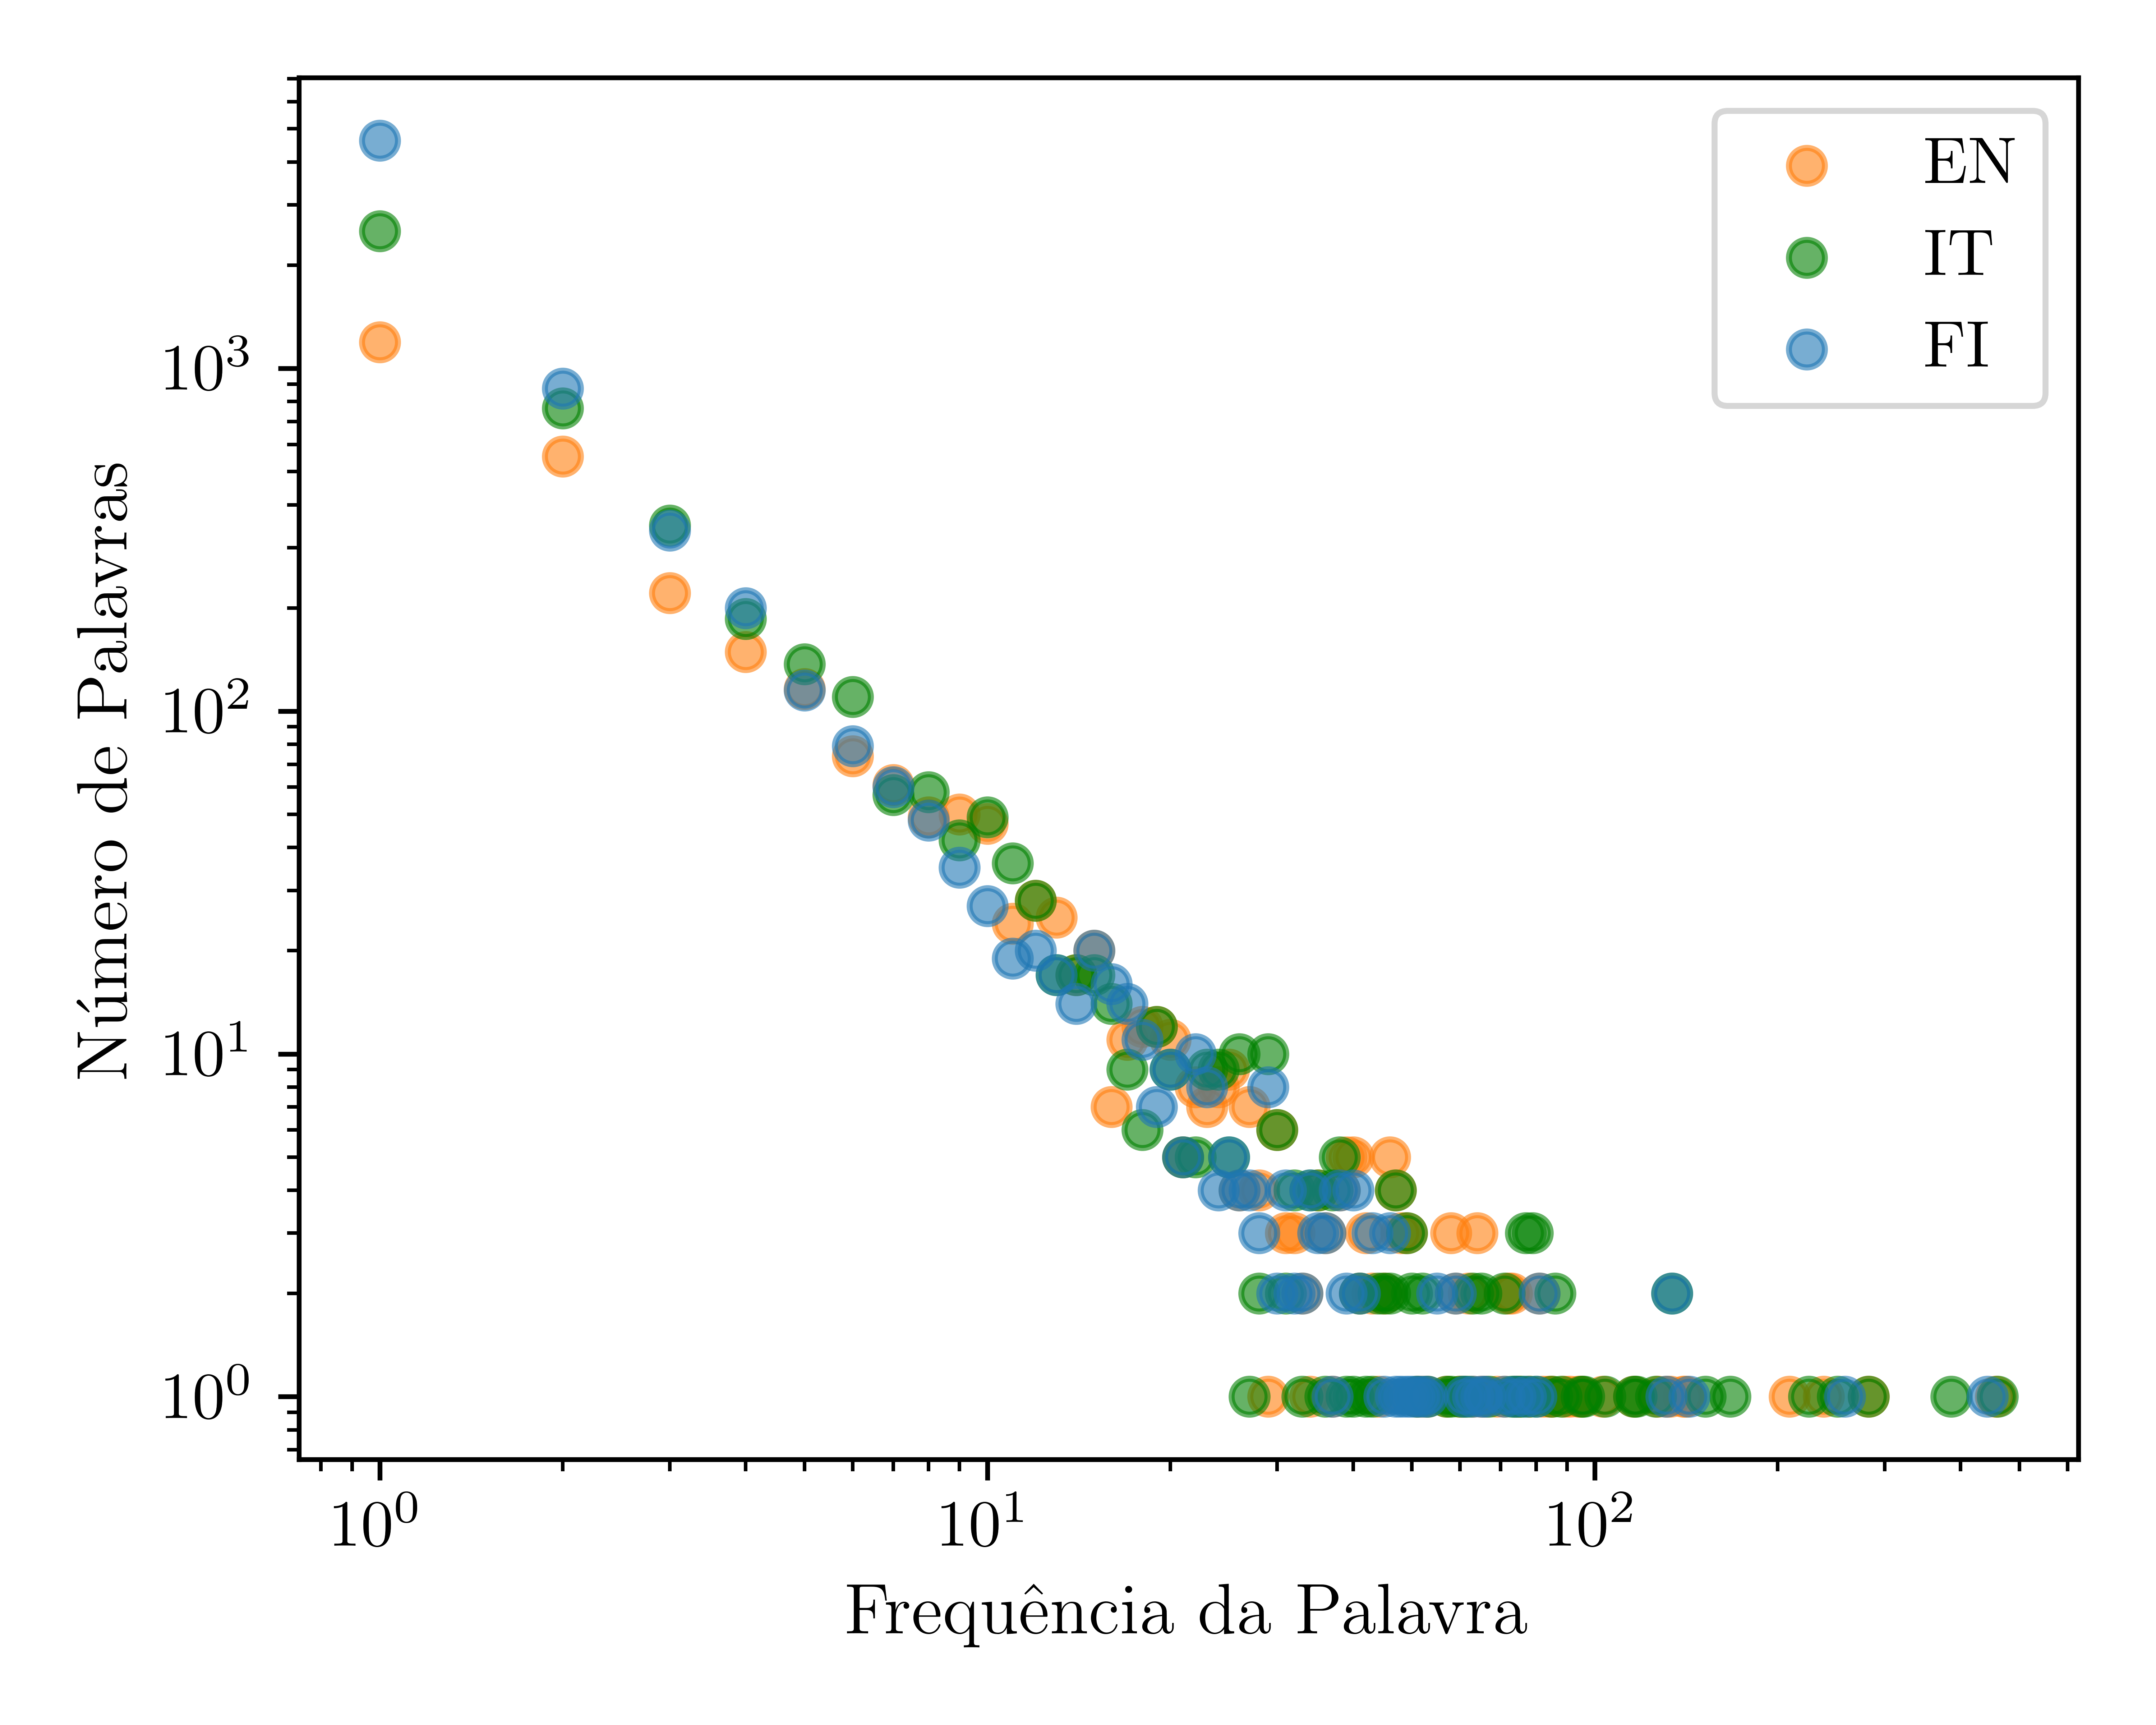
\includegraphics[width=0.45\textwidth]{../assets/exact_word_freqs.png}
    \caption{Distribuição da frequência de palavras, por idioma.}
    \label{fig:word_freqs}
\end{figure}

Por fim, ainda através da aplicação do algoritmo de contagem exata, torna-se possível a análise da quantidade de palavras distintas em cada idioma, como apresentado na Fig. \ref{fig:distinc_words}. Neste caso, é possível observar que a quantidade aumenta de idioma para idioma, inglês (EN) $<$ italiano (IT) $<$ finlandês (FI), o que pode não representar uma distinção entre as traduções, pelo facto deste desequilíbrio poder ser influenciado por fatores como a complexidade da língua ou o desempenho do \textit{spaCy} na lematização das palavras.

\begin{figure}[H]
    \centering
    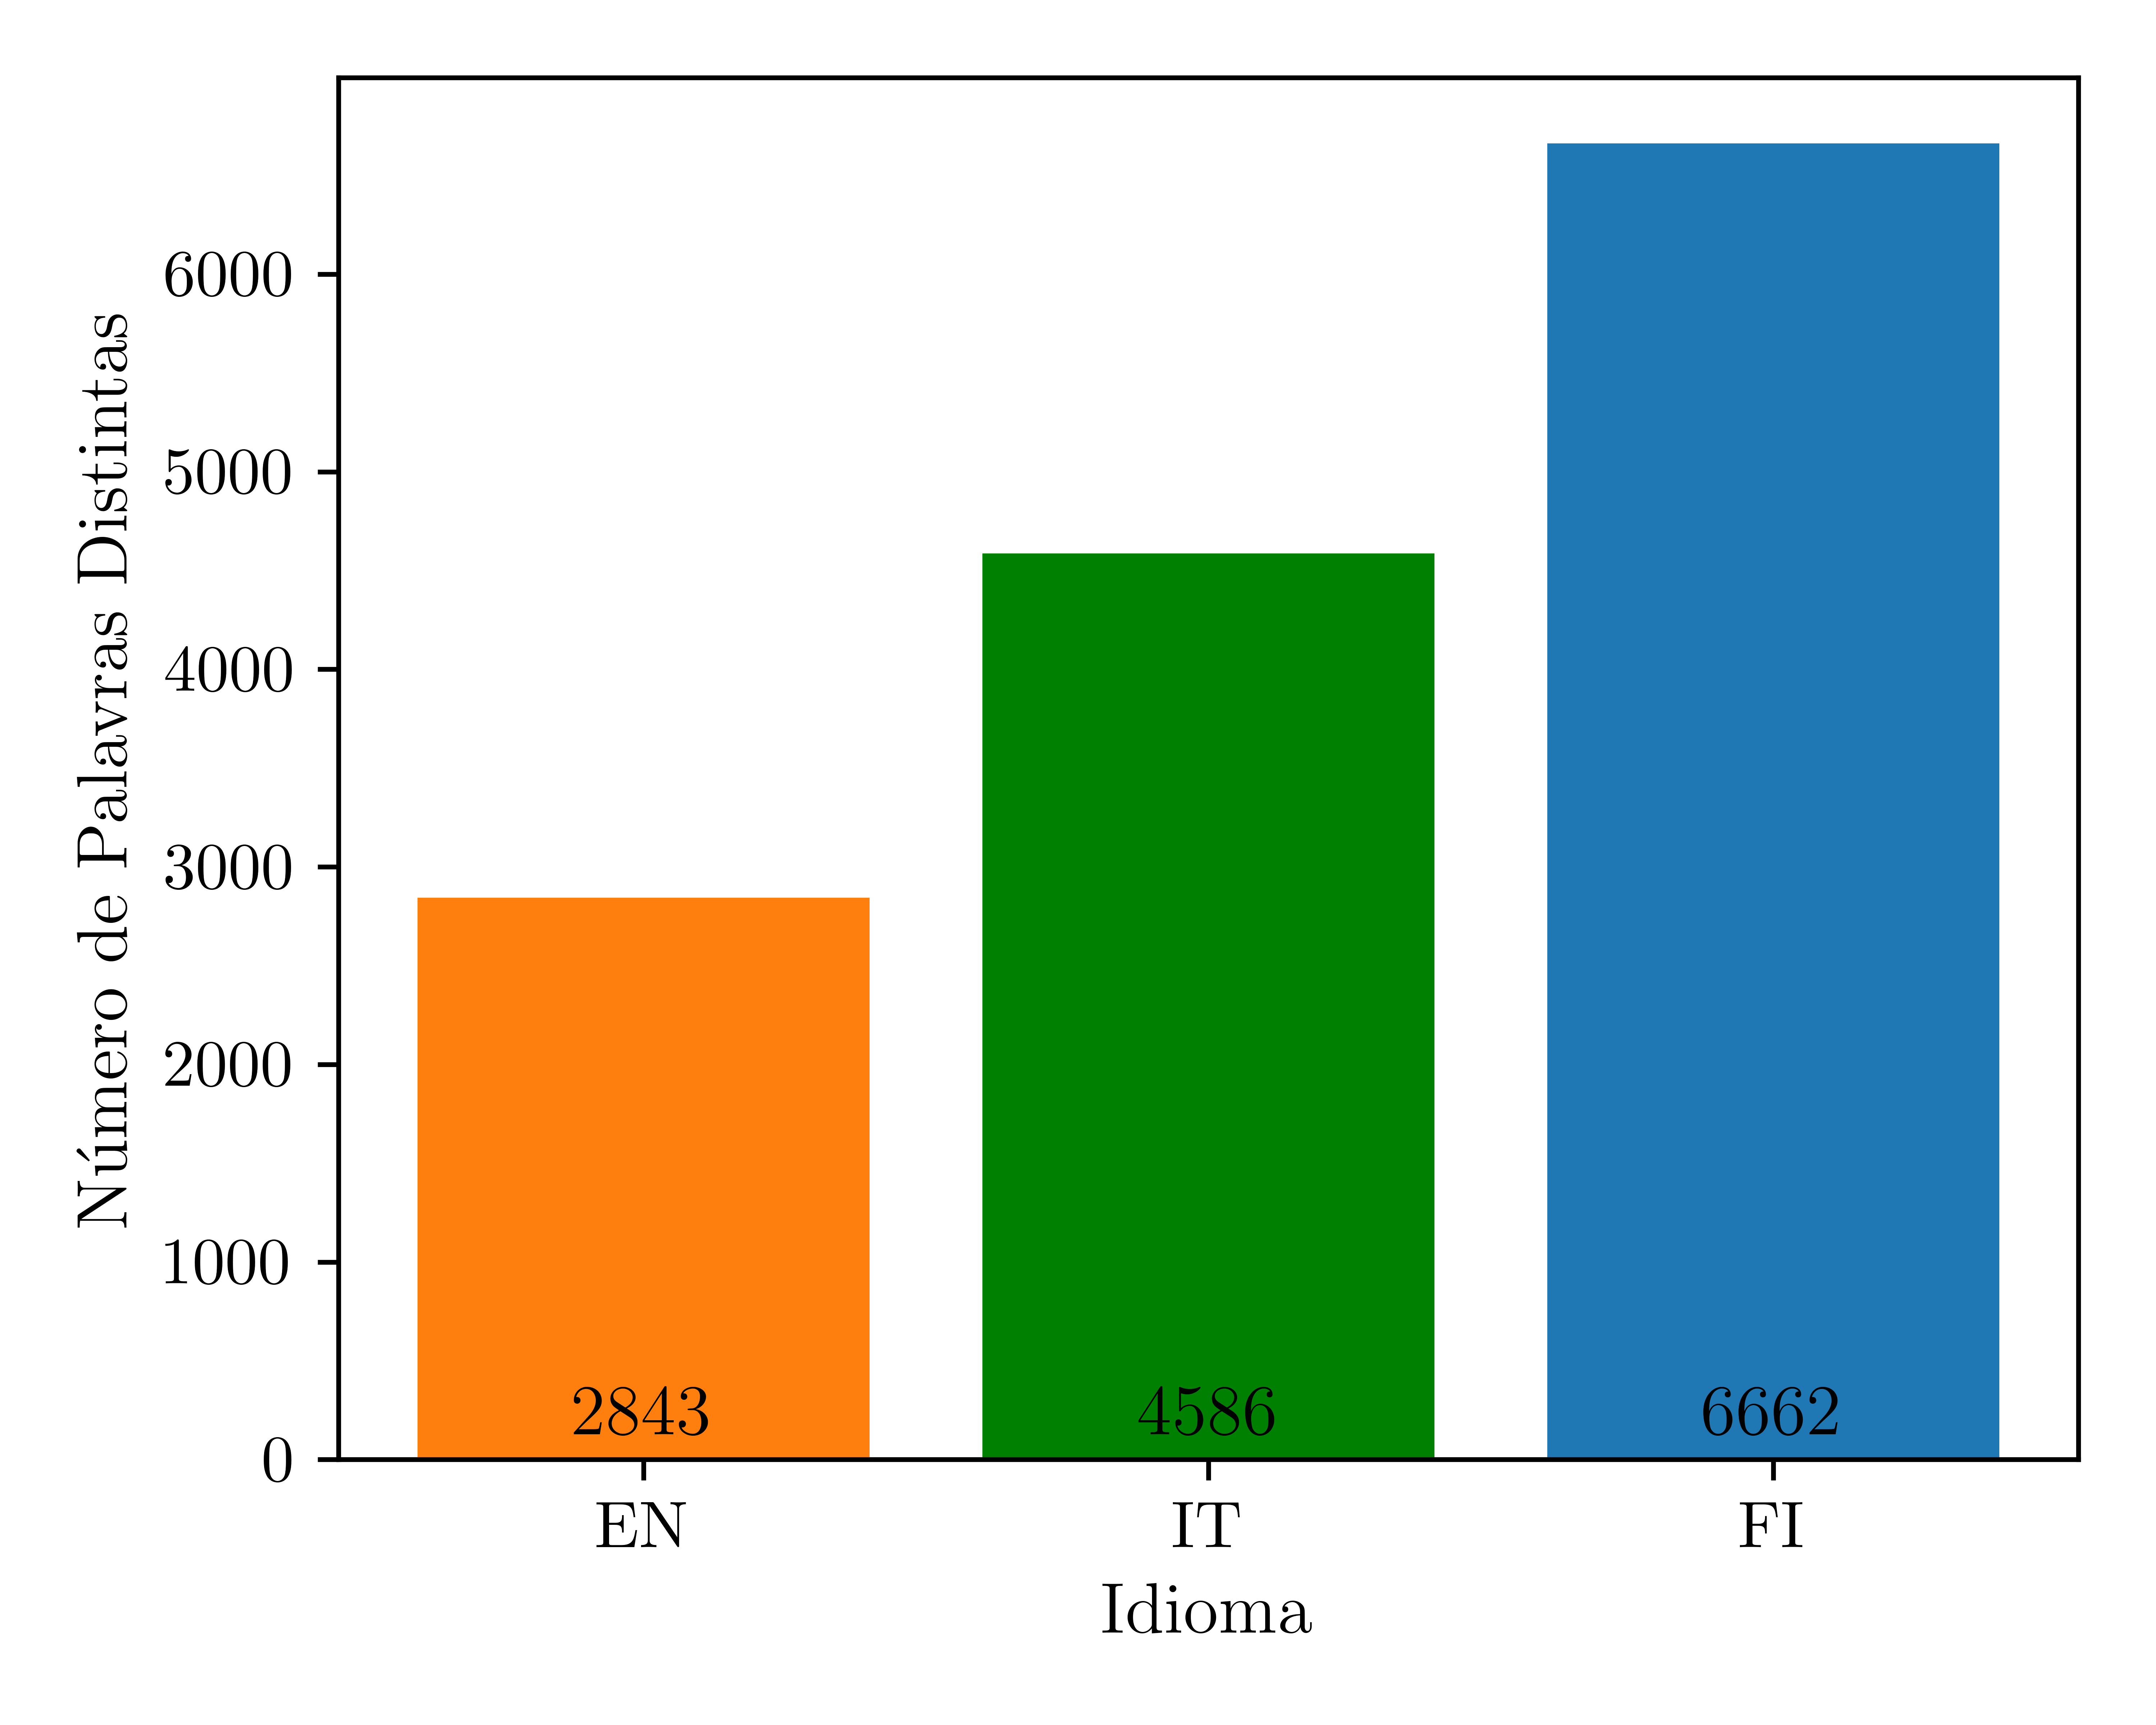
\includegraphics[width=0.45\textwidth]{../assets/exact_distinct_words.png}
    \caption{Número de palavras distintas analisadas pelo algoritmo, em cada idioma.}
    \label{fig:distinc_words}
\end{figure}

\section{Contadores Aproximados}

Os contadores aproximados, também conhecidos por contadores probabilísticos, inventados por Robert Morris, são algoritmos especializados em realizar estimativas eficientes de contagens, utilizando quantidades reduzidas de memória em comparação com métodos tradicionais, através de técnicas baseadas em probabilidade. Estes contadores são particularmente úteis em situações em que a precisão exata da contagem não é crítica, permitindo uma redução significativa no uso de memória, sem comprometer a qualidade da análise \cite{RM78}.

Um exemplo de um contador aproximado é o algoritmo de contagem aproximada apresentado de seguida, designado por \textit{Contador Aproximado}. Neste exemplo, o algoritmo utiliza uma probabilidade de contagem fixa de $1/16$, pelo que apenas é estudado um caso particular deste tipo de algoritmos neste relatório. Para cada evento, neste caso, cada palavra do texto, é gerado um número aleatório entre 0 e 1, sendo a palavra contada se o número gerado for menor que a probabilidade de contagem. Isto permite que a contagem seja realizada de forma aproximada, com uma margem de erro controlada e um menor uso de memória.

\begin{algorithm}[H]
\raggedright
\textbf{Entrada:} texto processado (\texttt{T}) \\
\textbf{Saída:} dicionário onde as palavras são as chaves e os valores são as suas frequências estimadas (\texttt{D})\\
\hrule 
\caption{Contador Aproximado}
\begin{algorithmic}[1]
    \State \texttt{D} $\gets$ empty dictionary
    \State \texttt{words} $\gets$ list of words from \texttt{T}
    \For{each \texttt{word} in \texttt{words}}
    \State \texttt{r} $\gets$ Uniform(0, 1)
    \If{$r < \frac{1}{16}$}
        \If{\texttt{word} $\not\in$ \texttt{D}}
            \State \texttt{D}[\texttt{word}] $\gets$ 0
        \EndIf
        \State \texttt{D}[\texttt{word}] $\gets$ \texttt{D}[\texttt{word}] + $1$
    \EndIf
    \EndFor
    \For{each \texttt{word} in \texttt{D}} \Comment{Estimate the total count}
    \State \texttt{D}[\texttt{word}] $\gets$ \texttt{D}[\texttt{word}] $\times 16$
    \EndFor
    \State \Return \texttt{D}
\end{algorithmic}
\end{algorithm}

Pelo facto deste algoritmo ter uma componente aleatória, para a obtenção dos resultados relativos ao mesmo, esta abordagem foi aplicada a cada livro em análise 20 vezes. Posteriormente, para cada uma das traduções, foi calculada a contagem (\#) mínima, média e máxima das palavras, sendo selecionadas as 10 palavras mais frequentes com base na média, de modo a obter uma estimativa das palavras mais frequentes em cada idioma. Estas contagens, tal como a contagem exata ($\text{\#}_\text{real}$), são apresentadas nas seguintes tabelas (Tabela \ref{table:top10_aprox_ingles} a \ref{table:top10_aprox_finlandes}). Nestas tabelas, para além das contagens referidas, também é possível verificar um código de cores nas palavras, preto, laranja e vermelho, que indicam se a posição da palavra está correta na ordem das 10 palavras mais frequentes, se está deslocada, ou se não faz parte das 10 mais frequentes de todo, respetivamente.

\begin{table}[H]
\centering
\caption{Estimativa das 10 palavras mais frequentes, pelo algoritmo de contagem aproximada, para o livro em inglês (IN).}
\label{table:top10_aprox_ingles}
\begin{tabular}{lrrr|r}
\toprule
Palavra & $\text{\#}_{\text{min}}$ & $\text{\#}_{\text{média}}$ & $\text{\#}_{\text{max}}$ & $\text{\#}_{\text{real}}$ \\
\midrule
pinocchio & 336 & 439 & 544 & 457 \\
say & 96 & 270 & 400 & 282 \\
little & 144 & 227 & 320 & 238 \\
puppet & 128 & 223 & 336 & 209 \\
come & 64 & 148 & 240 & 141 \\
boy & 80 & 140 & 176 & 140 \\
\textcolor{orange}{go} & 48 & 132 & 240 & 116 \\
\textcolor{orange}{poor} & 48 & 129 & 240 & 127 \\
\textcolor{orange}{like} & 32 & 128 & 192 & 133 \\
\textcolor{orange}{good} & 64 & 126 & 224 & 131 \\
\bottomrule
\end{tabular}
\end{table}

\begin{table}[H]
\centering
\caption{Estimativa das 10 palavras mais frequentes, pelo algoritmo de contagem aproximada, para o livro em italiano (IT).}
\label{table:top10_aprox_italiano}
\begin{tabular}{lrrr|r}
\toprule
Palavra & $\text{\#}_{\text{min}}$ & $\text{\#}_{\text{média}}$ & $\text{\#}_{\text{max}}$ & $\text{\#}_{\text{real}}$ \\
\midrule
pinocchio & 240 & 439 & 544 & 460 \\
il & 224 & 379 & 512 & 386 \\
dire & 160 & 263 & 448 & 282 \\
si & 128 & 252 & 320 & 251 \\
burattino & 96 & 223 & 320 & 225 \\
volere & 96 & 169 & 256 & 167 \\
\textcolor{orange}{povero} & 32 & 139 & 240 & 134 \\
\textcolor{red}{bello} & 80 & 133 & 240 & 116 \\
\textcolor{orange}{vedere} & 32 & 131 & 192 & 152 \\
\textcolor{orange}{andare} & 80 & 127 & 192 & 134 \\
\bottomrule
\end{tabular}
\end{table}

\begin{table}[H]
\centering
\caption{Estimativa das 10 palavras mais frequentes, pelo algoritmo de contagem aproximada, para o livro em finlandês (FI).}
\label{table:top10_aprox_finlandes}
\begin{tabular}{lrrr|r}
\toprule
Palavra & $\text{\#}_{\text{min}}$ & $\text{\#}_{\text{média}}$ & $\text{\#}_{\text{max}}$ & $\text{\#}_{\text{real}}$ \\
\midrule
pinocchio & 320 & 445 & 672 & 443 \\
sanoa & 160 & 266 & 352 & 258 \\
saada & 48 & 160 & 256 & 143 \\
tehdä & 48 & 136 & 224 & 134 \\
\textcolor{orange}{marionetti} & 80 & 132 & 224 & 131 \\
\textcolor{orange}{alkaa} & 64 & 104 & 160 & 134 \\
\textcolor{red}{geppetto} & 32 & 87 & 160 & 71 \\
huutaa & 32 & 86 & 128 & 81 \\
\textcolor{red}{pää} & 32 & 80 & 128 & 65 \\
\textcolor{red}{olla} & 16 & 76 & 144 & 61 \\
\bottomrule
\end{tabular}
\end{table}

Assim, é possível verificar que este algoritmo é tanto melhor quanto maior é a contagem real da palavra, o que se deve ao facto de haver uma menor densidade de palavras com contagens próximas, como foi verificado na contagem exata (Fig. \ref{fig:word_freqs}) e ao facto da probabilidade de contagem ser fixa, o que implica que a contagem de palavras com contagens mais baixas seja menos precisa.

\section{Contadores Space-Saving}

Pelo facto de muitos processos de geração de dados poderem ser modelados como fluxos de dados, que produzem enormes quantidades de informações simples isoladamente, mas que, em conjunto, formam um todo complexo, torna-se interessante a utilização de métodos que respondam rapidamente a cada nova informação e utilizem recursos muito pequenos em comparação com o volume total de dados. Neste contexto, o algoritmo de contagem \textit{Space-Saving} é uma solução eficiente para a identificação de itens frequentes em \textit{streams} de dados, permitindo acompanhar contagens frequentes de forma eficiente, mesmo sob restrições de memória (número máximo de diferentes palavras a manter, $k$) \cite{CG09}.

Este algoritmo é exposto no pseudocódigo seguinte:

\begin{algorithm}[H]
\raggedright
\textbf{Entrada:} \\
- texto processado (\texttt{T}) \\
- número máximo de itens a manter (\texttt{k}) \\
\textbf{Saída:} dicionário com a estimativa das \texttt{k} palavras mais frequentes e respetivas frequências estimadas (\texttt{D}) \\
\hrule 
\caption{Contador \textit{Space-Saving} \cite{CG09}}
\begin{algorithmic}[1]
    \State \texttt{D} $\gets$ empty dictionary
    \State \texttt{words} $\gets$ list of words from \texttt{T}
    \For{each \texttt{word} in \texttt{words}}
        \If{\texttt{word} $\in$ \texttt{D}}
            \State \texttt{D}[\texttt{word}] $\gets$ \texttt{D}[\texttt{word}] + $1$
        \ElsIf{$|\texttt{D}| < \texttt{k}$}
            \State \texttt{D}[\texttt{word}] $\gets$ $1$
        \Else
            \State \texttt{j} $\gets$ $\arg \min_{j \in \texttt{D}}\ \texttt{D}[\texttt{j}]$
            \State \texttt{D}[\texttt{word}] $\gets$ \texttt{D}[\texttt{j}] + $1$
            \State \texttt{D} $\gets$ \texttt{D} $\setminus \{\texttt{j}\}$
        \EndIf
    \EndFor
    \State \Return \texttt{D}
\end{algorithmic}
\end{algorithm}

Pelo facto deste algoritmo ser sensível ao valor de $k$, torna-se importante a realização de uma análise para a determinação do valor mínimo de $k$ que permita a obtenção de resultados precisos, neste caso das 10 palavras mais frequentes, sem comprometer a eficiência espacial do algoritmo \cite{ZF22}. Na Tabela \ref{table:top10_ss10} pode-se observar um exemplo de aplicação do algoritmo em análise, para um valor $k$ inadequado.

\begin{table}[H]
\centering
\caption{Estimativa das 10 palavras mais frequentes, pelo algoritmo de contagem \textit{Space-Saving}, com $k = 10$, para as traduções em inglês e finlandês.}
\label{table:top10_ss10}
\begin{tabular}{lr|lr}
\toprule
\multicolumn{2}{c}{EN} & \multicolumn{2}{c}{FI} \\
Palavra & \# & Palavra & \# \\
\midrule
boy & 1714 & poja & 1808 \\
time & 1713 & tyytyväinen & 1807 \\
say & 1713 & olinpa & 1807 \\
great & 1713 & sentään & 1807 \\
complacency & 1713 & hullunkurinen & 1807 \\
ridiculous & 1713 & näköinen & 1807 \\
puppet & 1713 & marionetti & 1807 \\
glad & 1713 & onnellinen & 1807 \\
behave & 1713 & muuttua & 1807 \\
little & 1713 & oikeaksi & 1807 \\
\bottomrule
\end{tabular}
\end{table}

Verifica-se que, quando o $k$ é $10$, todas as contagens têm o mesmo valor ($k/n$, onde $n$ é o número total de palavras), aproximadamente, o que não corresponde à realidade. Isto deve-se ao facto de o $k$ ser demasiado pequeno, e como tal, o algoritmo não consegue manter uma contagem precisa das palavras mais frequentes.

Tendo em vista a determinação do valor mínimo de $k$, com o objetivo de determinar os 10 itens mais frequentes, foi criada uma medida de contagens significativas, que consiste no número de contagens que estão a uma distância significativa do valor $k/n$, neste caso, de pelo menos $1\%$. A Fig. \ref{fig:meaningful_wordscount_k} apresenta a quantidade de palavras significativas em função de $k$, para o idioma italiano, e uma linha horizontal que representa o valor $10$, o número de palavras a identificar. Assim, é esperado que o $k$ mínimo seja o valor mais baixo que permita a identificação de pelo menos 10 palavras significativas (primeiro ponto acima da linha). É também importante referir que, ainda a partir da visualização, é possível observar a proporção entre $k$ e o número total de palavras ($n$) (eixo superior), para cada $k$, permitindo uma perceção da eficiência espacial do algoritmo.

\begin{figure}[H]
    \centering
    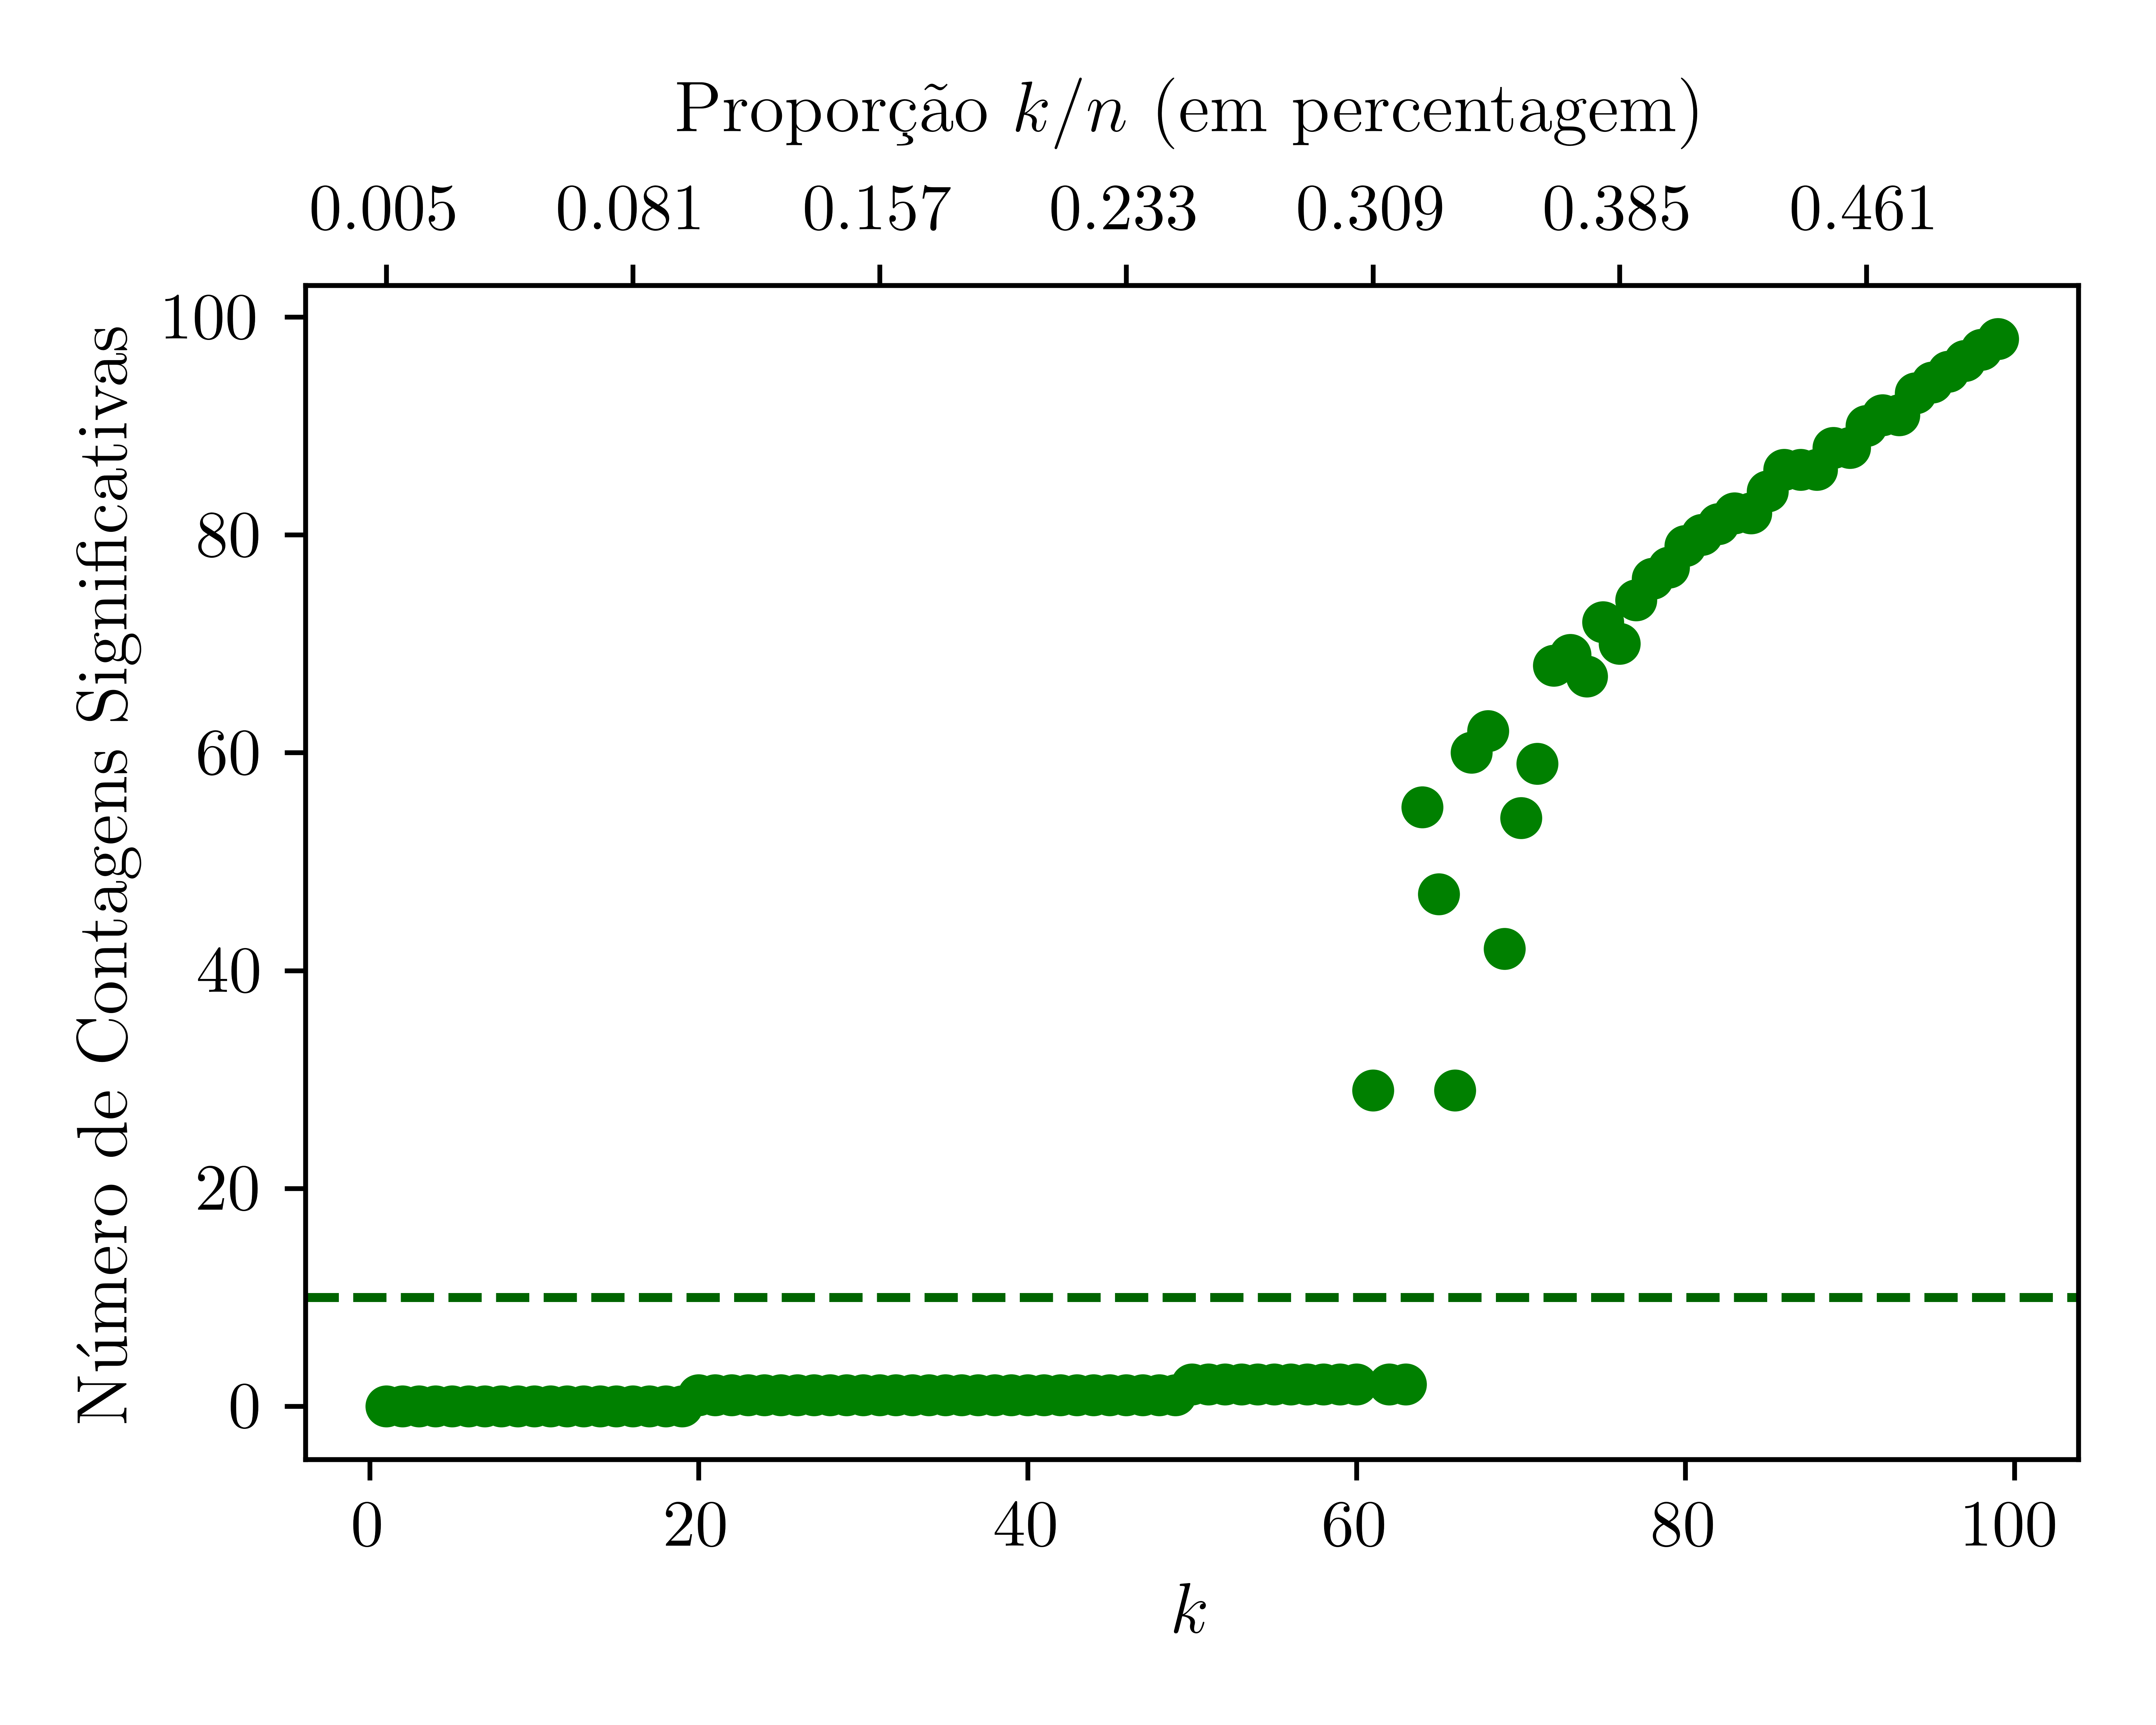
\includegraphics[width=0.45\textwidth]{../assets/ss_signcount.png}
    \caption{Número de palavras significativas em função do valor de $k$, para a tradução em italiano.}
    \label{fig:meaningful_wordscount_k}
\end{figure}

Através de uma análise numérica, com a metodologia referida, envolvendo o número de palavras significativas, foi possível determinar o valor mínimo de $k$ para cada uma das traduções, sendo estes apresentados na Tabela \ref{table:min_k_for_SStop10}.

\begin{table}[H]
\centering
\caption{Valor mínimo de $k$ para que o número de palavras significativas seja superior a 10, para cada tradução.}
\label{table:min_k_for_SStop10}
\begin{tabular}{cc|cc|cc}
\toprule
\multicolumn{2}{c}{EN} & \multicolumn{2}{c}{IT} & \multicolumn{2}{c}{FI} \\
$k$ & $k/n$ & $k$ & $k/n$ & $k$ & $k/n$ \\
\midrule
$59$ & $0.344\%$ & $61$ & $0.309\%$ & $67$ & $0.371\%$ \\
\bottomrule
\end{tabular}
\end{table}

Pelo facto de todos os valores de $k$ obtidos a partir da análise da tabela anterior serem próximos e não representarem um valor significativo de memória, foi selecionado o valor $k = 70$ para a aplicação do algoritmo de contagem \textit{Space-Saving} a todos os livros em análise. A Tabela \ref{table:top10_ss70} apresenta as 10 palavras mais frequentes em cada um dos livros, com base na aplicação do algoritmo com $k = 70$, juntamente com a sua contagem estimada, e um código de cores nas palavras, que indica se a posição da palavra está correta na ordem das 10 palavras mais frequentes (preto), se está deslocada (laranja) ou se não faz parte das 10 mais frequentes de todo (vermelho).

\begin{table}[H]
\centering
\caption{Estimativa das 10 palavras mais frequentes, pelo algoritmo de contagem \textit{Space-Saving}, com $k = 70$.}
\label{table:top10_ss70}
\begin{tabular}{lr|lr|lr}
\toprule
\multicolumn{2}{c}{EN} & \multicolumn{2}{c}{IT} & \multicolumn{2}{c}{FI} \\
Palavra & \# & Palavra & \# & Palavra & \# \\
\midrule
pinocchio & 457 & pinocchio & 466 & pinocchio & 443 \\
say & 288 & il & 389 & sanoa & 266 \\
little & 270 & dire & 283 & \textcolor{red}{pieni} & 257 \\
\textcolor{orange}{good} & 244 & \textcolor{orange}{burattino} & 283 & \textcolor{red}{geppetto} & 257 \\
\textcolor{red}{snail} & 243 & \textcolor{red}{pesce} & 280 & \textcolor{red}{ihmeellinen} & 256 \\
\textcolor{red}{fairy} & 243 & \textcolor{orange}{si} & 279 & \textcolor{red}{isä} & 256 \\
\textcolor{red}{new} & 242 & \textcolor{orange}{ragazzo} & 279 & \textcolor{red}{vanha} & 256 \\
\textcolor{orange}{boy} & 242 & \textcolor{red}{ciuchino} & 279 & \textcolor{red}{istua} & 256 \\
\textcolor{red}{look} & 242 & \textcolor{red}{geppetto} & 278 & \textcolor{red}{pää} & 256 \\
\textcolor{red}{geppetto} & 242 & \textcolor{red}{fata} & 278 & \textcolor{red}{äkkinäinen} & 256 \\
\bottomrule
\end{tabular}
\end{table}

Pelo facto dos resultados obtidos com o algoritmo de contagem \textit{Space-Saving} com $k = 70$ não serem suficientemente precisos, devido ao valor de $k$ e por existirem várias contagens muito próximas nas 10 palavras mais frequentes, pode-se concluir que a medida de contagens significativas poderá ter de ser melhorada, possivelmente aumentando a distância que determina a significância de uma contagem.

Não sendo a determinação desta medida o foco deste estudo, foi selecionado empiricamente um valor de $k = 150$, tendo em vista uma melhoria na precisão das contagens. Na Tabela \ref{table:top10_ss150} são apresentadas as 10 palavras mais frequentes em cada um dos livros, com base na aplicação do algoritmo com $k = 150$, juntamente com a sua contagem estimada, e um código de cores nas palavras, com a mesma finalidade apresentada nas tabelas anteriores.

\begin{table}[H]
\centering
\caption{Estimativa das 10 palavras mais frequentes, pelo algoritmo de contagem \textit{Space-Saving}, com $k = 150$.}
\label{table:top10_ss150}
\begin{tabular}{lr|lr|lr}
\toprule
\multicolumn{2}{c}{EN} & \multicolumn{2}{c}{IT} & \multicolumn{2}{c}{FI} \\
Palavra & \# & Palavra & \# & Palavra & \# \\
\midrule
pinocchio & 457 & pinocchio & 461 & pinocchio & 443 \\
say & 284 & il & 386 & sanoa & 261 \\
little & 239 & dire & 282 & saada & 143 \\
puppet & 209 & si & 251 & \textcolor{orange}{marionetti} & 138 \\
\textcolor{orange}{boy} & 150 & burattino & 225 & \textcolor{orange}{alkaa} & 136 \\
\textcolor{orange}{come} & 145 & volere & 168 & \textcolor{orange}{tehdä} & 135 \\
\textcolor{orange}{good} & 135 & vedere & 152 & \textcolor{red}{isä} & 128 \\
\textcolor{red}{donkey} & 134 & \textcolor{orange}{ragazzo} & 145 & \textcolor{red}{pieni} & 121 \\
\textcolor{orange}{like} & 133 & \textcolor{red}{bello} & 138 & \textcolor{red}{päivä} & 119 \\
go & 129 & \textcolor{orange}{andare} & 137 & \textcolor{red}{pois} & 119 \\
\bottomrule
\end{tabular}
\end{table}

Observa-se que, com o aumento do valor de $k$, a precisão das contagens aumenta significativamente, sendo possível identificar as 10 palavras mais frequentes com maior precisão, em comparação com os resultados obtidos com $k = 70$. No entanto, ainda existem algumas palavras que não estão corretamente posicionadas.

Isto revela que quanto maior o valor de $k$, maior a precisão das contagens, no entanto, também maior o uso de memória. Assim, é importante encontrar um equilíbrio entre a precisão das contagens e a eficiência espacial do algoritmo, de modo a obter resultados precisos sem comprometer a eficiência do mesmo.

\section{Resultados}

\subsection{Análise da Classicação das Palavras Frequentes}

Tendo em conta que ao longo deste relatório foram apresentadas as 10 palavras mais frequentes em cada um dos livros e respetivas contagens, com base na aplicação dos diferentes algoritmos, torna-se interessante a análise da posição de cada palavra em relação à sua posição real.

Nas Tabelas \ref{table:rank10_ing}, \ref{table:rank10_it} e \ref{table:rank10_fi} são apresentadas as 10 palavras mais frequentes em cada uma das traduções (EN, IT e FI, respetivamente) e para cada palavra é apresentada a classificação obtida com a aplicação de cada um dos algoritmos. Nas mesmas tabelas, é também apresentado o número de palavras corretamente classificadas, ou seja, que se encontram na posição correta.

\begin{table}[H]
\centering
\caption{10 palavras mais frequentes em inglês, com a classificação obtida a partir da aplicação de cada algoritmo.}
\label{table:rank10_ing}
\begin{tabular}{lrrrrr}
\toprule
Palavra & Exato & Aprox. & SS10 & SS70 & SS150 \\
\midrule
pinocchio & 1 & 1 & - & 1 & 1 \\
say & 2 & 2 & 3 & 2 & 2 \\
little & 3 & 3 & 10 & 3 & 3 \\
puppet & 4 & 4 & 7 & 20 & 4 \\
come & 5 & 5 & - & - & 6 \\
boy & 6 & 6 & 1 & 8 & 5 \\
like & 7 & 9 & - & - & 9 \\
good & 8 & 10 & - & 4 & 7 \\
poor & 9 & 8 & - & - & 11 \\
go & 10 & 7 & - & 11 & 10 \\
\midrule
Corretas & 10 & 6 & 0 & 3 & 5 \\
\bottomrule
\end{tabular}
\end{table}

\begin{table}[H]
\centering
\caption{10 palavras mais frequentes em italiano, com a classificação obtida a partir da aplicação de cada algoritmo.}
\label{table:rank10_it}
\begin{tabular}{lrrrrr}
\toprule
Palavra & Exato & Aprox. & SS10 & SS70 & SS150 \\
\midrule
pinocchio & 1 & 1 & - & 1 & 1 \\
il & 2 & 2 & - & 2 & 2 \\
dire & 3 & 3 & - & 3 & 3 \\
si & 4 & 4 & - & 6 & 4 \\
burattino & 5 & 5 & - & 4 & 5 \\
volere & 6 & 6 & - & - & 6 \\
vedere & 7 & 9 & - & - & 7 \\
andare & 8 & 10 & - & - & 10 \\
povero & 9 & 7 & - & - & 12 \\
ragazzo & 10 & 12 & - & 7 & 8 \\
\midrule
Corretas & 10 & 6 & 0 & 3 & 7 \\
\bottomrule
\end{tabular}
\end{table}

\begin{table}[H]
\centering
\caption{10 palavras mais frequentes em finlandês, com a classificação obtida a partir da aplicação de cada algoritmo.}
\label{table:rank10_fi}
\begin{tabular}{lrrrrr}
\toprule
Palavra & Exato & Aprox. & SS10 & SS70 & SS150 \\
\midrule
pinocchio & 1 & 1 & - & 1 & 1 \\
sanoa & 2 & 2 & - & 2 & 2 \\
saada & 3 & 3 & - & 47 & 3 \\
alkaa & 4 & 6 & - & 24 & 5 \\
tehdä & 5 & 4 & - & 25 & 6 \\
marionetti & 6 & 5 & 7 & 19 & 4 \\
poika & 7 & 14 & - & - & 17 \\
huutaa & 8 & 8 & - & - & 135 \\
nähdä & 9 & 12 & - & - & 13 \\
kysyä & 10 & 11 & - & - & 14 \\
\midrule
Corretas & 10 & 4 & 0 & 2 & 3 \\
\bottomrule
\end{tabular}
\end{table}

É possível verificar um desempenho semelhante dos algoritmos entre os diferentes idiomas, apesar do idioma finlandês apresentar um desempenho ligeiramente inferior, o que pode ser justificado pela maior quantidade de palavras distintas, como foi verificado na análise da contagem exata (Fig. \ref{fig:distinc_words}). Para além disso, também se observa um mau resultado dos algoritmos de \textit{Space-Saving} com $k = 10$ e $k = 70$, um resultado satisfatório com os algoritmos de contagem aproximada e \textit{Space-Saving} com $k = 150$ e um resultado perfeito com o algoritmo de contagem exata.

\subsection{Análise de Precisão}

De forma a avaliar a precisão das contagens obtidas com a aplicação dos diferentes algoritmos, foi realizada uma análise ao erro relativo, dado por
$$
\frac{\sum^{10}_{\text{Palavra} = 1} | \text{Cont.Est.}_{\text{Palavra}} - \text{Cont.Real}_{\text{Palavra}} | }{\sum^{10}_{\text{Palavra} = 1} \text{Cont.Real}_{\text{Palavra}}\ /\ 10}
$$
para cada um dos diferentes algoritmos e livros em análise. É de notar que este erro apenas considera as 10 palavras mais frequentes de cada livro, uma vez que estas são o foco da análise, e pelo facto do algoritmo de \textit{Space-Saving}, com $k = 10$, apenas manter as contagens de 10 palavras. A Tabela \ref{table:erro_relativo} apresenta os resultados referentes a esta análise.

\begin{table}[H]
\centering
\caption{Erro relativo das contagens obtidas com a aplicação dos diferentes algoritmos, para cada livro.}
\label{table:erro_relativo}
\begin{tabular}{lrrrrr}
\toprule
& Exato & Aprox. & SS10 & SS70 & SS150 \\
\midrule
EN & 0.000 & 0.047 & 3.571 & 0.598 & 0.026 \\
IT & 0.000 & 0.043 & 1.000 & 0.561 & 0.019 \\
FI & 0.000 & 0.078 & 2.179 & 0.757 & 0.198 \\
\bottomrule
\end{tabular}
\end{table}

Observa-se que o algoritmo de contagem exata é o que apresenta um menor erro relativo, uma vez que mantém a contagem exata de todas as palavras, o que permite uma maior precisão. Por outro lado, os algoritmos de contagem aproximada e \textit{Space-Saving} apresentam um erro relativo superior, uma vez que utilizam técnicas probabilísticas e de limitação de memória, respetivamente, para manter as contagens de palavras, o que implica uma menor precisão. Particularmente, o algoritmo de contagem \textit{Space-Saving} é o que apresenta um maior erro relativo, quando tem um menor valor de $k$, uma vez que mantém apenas as contagens de $k$ palavras, levando a uma menor precisão.

\subsection{Análise de Memória}

Sendo a componente espacial um dos fatores mais importantes na análise de algoritmos de contagem, torna-se fundamental uma análise da quantidade de memória utilizada por cada um dos algoritmos em análise.

Para tal, foi realizada uma comparação da memória alocada para manter as contagens de palavras, para cada um dos algoritmos e livros em análise. A Tabela \ref{table:memoria} apresenta esta comparação, tendo sido a memória medida em \textit{bytes}, através da função \textit{asizeof}, do pacote \textit{pympler}, do \textit{Python}.

\begin{table}[H]
\centering
\caption{Memória utilizada por cada algoritmo, em \textit{bytes}, para cada livro.}
\label{table:memoria}
\begin{tabular}{lrrrrr}
\toprule
& Exato & Aprox. & SS10 & SS70 & SS150 \\
\midrule
EN & 525112 & 359432 & 7984 & 18832 & 33264 \\
IT & 865568 & 572312 & 8064 & 18992 & 33664 \\
FI &1332984 & 884776 & 8176 & 20000 & 35888 \\
\bottomrule
\end{tabular}
\end{table}

Observa-se que o algoritmo de contagem exata é o que requer uma maior quantidade de memória, uma vez que necessita de manter a contagem exata de todas as palavras, o que implica uma maior quantidade de informação a ser guardada. Por outro lado, os algoritmos de contagem aproximada e \textit{Space-Saving} requerem uma menor quantidade de memória, uma vez que utilizam técnicas probabilísticas e de limitação de memória, respetivamente, para manter as contagens de palavras. Particularmente, o algoritmo de contagem \textit{Space-Saving} é o que apresenta uma menor quantidade substancial de memória alocada, uma vez que mantém apenas as contagens de $k$ palavras, sendo que a memória alocada aumenta com o aumento de $k$.

\section{Conclusão}

Em suma, a análise de diferentes abordagens de contagem de palavras, nomeadamente a contagem exata, a contagem aproximada e a contagem \textit{Space-Saving}, permitiu a verificação da eficiência e precisão de cada qual, tendo em conta diferentes fatores, como a classificação das palavras mais frequentes, o erro relativo das contagens e a memória alocada para manter as contagens de palavras.

Verificou-se que o algoritmo de contagem exata é o que apresenta uma maior precisão, seguido dos algoritmos de contagem aproximada e \textit{Space-Saving}, com $k = 150$, que apresentam um desempenho próximo, e por fim, os algoritmos de \textit{Space-Saving} com $k = 70$ e $k=10$, que apresentam um desempenho inferior, respetivamente. 

Contudo, também se observou que são estes últimos algoritmos que apresentam uma menor quantidade de memória alocada, em comparação com os algoritmos de contagem exata e aproximada, que requerem uma maior quantidade de memória.

Estes resultados permitem concluir que, apesar do algoritmo de contagem exata apresentar uma maior precisão, este requer uma maior quantidade de memória, o que pode ser um fator limitante em análises com grandes volumes de dados. Por outro lado, os algoritmos de contagem aproximada e \textit{Space-Saving} apresentam uma menor precisão, mas requerem uma menor quantidade de memória, o que pode ser uma vantagem em análises com grandes volumes de dados.

Assim, é possível concluir que a escolha do algoritmo a utilizar deve ser feita tendo em conta um equilíbrio entre a precisão das contagens e a eficiência espacial do algoritmo, de modo a obter resultados precisos sem comprometer a eficiência do mesmo, pelo que consoante o objetivo da análise, a escolha do algoritmo a utilizar poderá variar.

\bibliography{refs}

\end{document}
